\documentclass[12pt]{article}

\usepackage{../thesis}

\usepackage{tikz} 

\begin{document}

\pagestyle{empty}

\begin{tikzpicture}
    \node[anchor=south west,inner sep=0] (image) at (0,0) {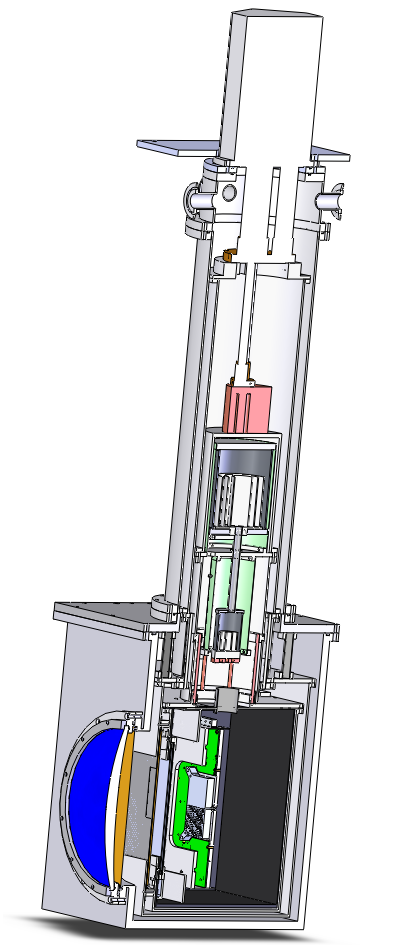
\includegraphics[width=2.4in]{../images/cryostat-cutaway.png}};
    \begin{scope}[x={(image.south east)},y={(image.north west)}]
	    %\draw[help lines,xstep=.1,ystep=.1] (0,0) grid (1.5,1);
		%\foreach \x in {0,1,...,15} { \node [anchor=north] at (\x/10,0) {0.\x}; }
		%\foreach \y in {0,1,...,9} { \node [anchor=east] at (0,\y/10) {0.\y}; }
		
        \draw[red,ultra thick,rounded corners] (0.50,0.7) rectangle (0.85,0.75) node[below left] {\textbf{A}}; % \PTC407 1st stage CH
        \draw[red,ultra thick,rounded corners] (0.56,0.595) rectangle (0.71,0.64) node[below left] {\textbf{B}}; % \PTC407 2st stage CH
        \draw[red,ultra thick,rounded corners] (0.53,0.55) rectangle (0.78,0.595) node[below left] {\textbf{C}}; % Cu Cylinder
        \draw[red,ultra thick,rounded corners] (0.505,0.32) rectangle (0.75,0.55) node at +(-0.1,-0.03) {\textbf{D}}; % sorp fridge
        \draw[red,ultra thick,rounded corners] (0.4,0.06) rectangle (0.70,0.26) node[red,below left] {\textbf{E}}; % Focal Plane
        
        \draw[thick,<->] (1.05,0.04) -- +(0,0.31) node[midway,right] {18 in}; % scale bar
    \end{scope}
\end{tikzpicture}

\end{document}
